\documentclass[10pt, a4paper, twoside, halfparskip, headsepline]{scrbook}
\usepackage[T1]{fontenc} % Umlaute
\usepackage[utf8]{inputenc} % Textcodierung
\usepackage[english]{babel} % Silbentrennung
%\usepackage{marvosym, amsmath, amssymb} % Symbole, Formeln, amssymb > mathdesign
\usepackage{lmodern, microtype} % enhanced CM, mikrotypografische Feinheiten
\usepackage[vmargin=3.4cm,hmargin=3cm]{geometry}
%\usepackage{graphicx} % Grafiken
%\usepackage{listings} % Quelltext
\usepackage[hidelinks]{hyperref} % Hyperlinks
%\usepackage[dvipsnames]{xcolor} % Farben (goo.gl/sP8iP, S.38)
%\usepackage[charter]{mathdesign} % Schriftart B. Charter
%\usepackage{mathptmx} % Schriftart Times
\usepackage[autolanguage]{numprint} % Zahlen

\usepackage{booktabs, tabularx} % Tabellen spacing/lines, linebreak/width
%\newcolumntype{Y}{>{\raggedright\arraybackslash}X}

\usepackage{csquotes} % Recommended addition for biblatex
\usepackage[style=numeric,backend=biber]{biblatex}
\addbibresource{thesis.bib}

\usepackage{caption}
\captionsetup{labelfont=bf,format=plain}

\usepackage[firstpage]{draftwatermark} % [final]
\SetWatermarkLightness{0.9}

\let\origunderscore\_
\renewcommand{\_}{\origunderscore\allowbreak}
\newcommand{\config}[1]{\texttt{config.\allowbreak #1}}

\begin{document}
\pagestyle{empty}
\pagenumbering{alph}
\begin{titlepage}
\begin{center}
\large{Lehrstuhl für IT-Sicherheitsinfrastrukturen, Informatik 1\\
Friedrich-Alexander-Universität Erlangen-Nürnberg}

\vspace{2cm}
\textbf{\Large{Bachelor Thesis}}

\vspace{1cm}
\textbf{\textsf{\huge{Analysis of BitTorrent Trackers and Peers}}}

\vspace{0.4cm}
\textbf{\textsf{\LARGE{Counting Confirmed Downloads in BitTorrent}}}

\vspace{1cm}
\Large{Stefan Schindler\footnote{Email: stefan@kaloix.de, Student number: 21676746}}

\vspace{1cm}
\Large{Erlangen, \today}

\vspace{6cm}
\large{Examiner: Prof. Dr.-Ing. Felix Freiling\\
Advisor: Philipp Klein, M. Sc. and Michael Gruhn}

\vspace{2cm}
\large{This work is licensed under the\\
Creative Commons Attribution-ShareAlike 4.0 International License.\\
To view a copy of this license, visit\\
\url{http://creativecommons.org/licenses/by-sa/4.0/}.}
\end{center}
\end{titlepage}
\cleardoublepage
%%%%%%%%%%%%%%%%%%%%%%%%%%%%%%%%%%%%%%%%%%%%%%%%%%%%%%%%%%%%%%%%%%%%%%%%%%%%%%%%%%

\pagestyle{plain}
\pagenumbering{roman}
\vspace*{\fill}
\section*{Eidesstattliche Erklärung / Statutory Declaration}

\vspace{0.1cm}
\noindent\hrule
\begin{quote}
Hiermit versichere ich eidesstattlich, dass die vorliegende Arbeit von mir
selbständig, ohne Hilfe Dritter und ausschließlich unter Verwendung der
angegebenen Quellen angefertigt wurde. Alle Stellen, die wörtlich oder
sinngemäß aus den Quellen entnommen sind, habe ich als solche kennt\-lich
gemacht. Die Arbeit wurde bisher in gleicher oder ähnlicher Form keiner anderen
Prüfungsbehörde vorgelegt.
\end{quote}

\begin{quote}
I hereby declare formally that I have developed and written the enclosed thesis
entirely by myself and have not used sources or means without declaration in
the text. Any thoughts or quotations which were inferred from the sources are
marked as such. This thesis was not submitted in the same or a substantially
similar version to any other authority to achieve an academic grading.
\end{quote}
\noindent\hrule

\vspace{0.5cm}
\noindent
Der Friedrich-Alexander-Universität, vertreten durch den Lehrstuhl
für Informatik 1, wird für Zwecke der Forschung und Lehre ein
einfaches, kostenloses, zeitlich und örtlich unbeschränktes
Nutzungsrecht an den Arbeitsergebnissen der Arbeit einschließlich
etwaiger Schutz- und Urheberrechte eingeräumt.

\vspace{0.5cm}
\noindent
Erlangen, \today

\vspace{1cm}
\begin{flushright}
Stefan Schindler \quad\null
\end{flushright}
\cleardoublepage
%%%%%%%%%%%%%%%%%%%%%%%%%%%%%%%%%%%%%%%%%%%%%%%%%%%%%%%%%%%%%%%%%%%%%%%%%%%%%%%%%%

\vspace*{\fill}
\begin{center}
{\large\textbf{Zusammenfassung}}
\end{center}

\begin{quote}
Zusammenfassung auf Deutsch
\end{quote}

\vspace*{\fill}
\begin{center}
{\large\textbf{Abstract}}
\end{center}

\begin{quote}
Zusammenfassung auf Englisch
\end{quote}
\vspace*{\fill}
%%%%%%%%%%%%%%%%%%%%%%%%%%%%%%%%%%%%%%%%%%%%%%%%%%%%%%%%%%%%%%%%%%%%%%%%%%%%%%%%%%

\tableofcontents
%%%%%%%%%%%%%%%%%%%%%%%%%%%%%%%%%%%%%%%%%%%%%%%%%%%%%%%%%%%%%%%%%%%%%%%%%%%%%%%%%%

\listoffigures
%%%%%%%%%%%%%%%%%%%%%%%%%%%%%%%%%%%%%%%%%%%%%%%%%%%%%%%%%%%%%%%%%%%%%%%%%%%%%%%%%%

\listoftables
%%%%%%%%%%%%%%%%%%%%%%%%%%%%%%%%%%%%%%%%%%%%%%%%%%%%%%%%%%%%%%%%%%%%%%%%%%%%%%%%%%

% Some general information on the context and setting
\chapter{Introduction}
\pagestyle{headings}
\pagenumbering{arabic}
\begin{table}
\centering
\begin{tabular}{llrrrr}
\toprule
& & \multicolumn{2}{c}{Upstream} & \multicolumn{2}{c}{Downstream} \\
\cmidrule{3-6}
Region & Access Type & Share & Volume & Share & Volume \\
\midrule
North America & fixed  & \numprint[\%]{25.49} & \numprint[MB]{2167} & \numprint[\%]{2.80} & \numprint[MB]{1369} \\
              & mobile & \numprint[\%]{1.88} & \numprint[MB]{1} & n/a & n/a \\
Europe        & fixed  & \numprint[\%]{36.56} & \numprint[MB]{1865} & \numprint[\%]{10.39} & \numprint[MB]{2400} \\
              & mobile & \numprint[\%]{8.99} & \numprint[MB]{6} & n/a & \numprint[MB]{11} \\
Latin America & fixed  & \numprint[\%]{23.87} & \numprint[MB]{454} & \numprint[\%]{7.42} & \numprint[MB]{913} \\
              & mobile & n/a & n/a & n/a & n/a \\
Asia-Pacific  & fixed  & \numprint[\%]{55.91} & \numprint[MB]{7492} & \numprint[\%]{22.78} & \numprint[MB]{7221} \\
              & mobile & \numprint[\%]{3.43} & \numprint[MB]{5} & n/a & n/a \\
Africa        & fixed  & \numprint[\%]{28.21} & n/a & \numprint[\%]{13.29} & n/a \\
              & mobile & \numprint[\%]{3.59} & n/a & \numprint[\%]{4.88} & n/a \\
\bottomrule
\end{tabular}
\caption[BitTorrent traffic per household, from \textsc{Sandvine}]{Share and volume per month of BitTorrent traffic per household, from \textsc{Sandvine} study \emph{Global Internet Phenomena Report 2H 2014} \cite{sandvine2014}. \emph{Share} percentages were determined by \textsc{Sandvine} and reportedly measured during ``peak period traffic'', see ``Top 10 Peak Period Applications''. \emph{Volume} values given above are an estimation based on BitTorrent's share in peak traffic and \textsc{Sandvine}'s mean value for overall ``Monthly Consumption'' per household. \emph{n/a} indicates BitTorrent is not among the top ten applications. No traffic volume is stated for Africa.}
\label{traffic}
\end{table}

% BitTorrent by Cohen, a decentralized network
In 2008, \textsc{Bram Cohen} published the specification for a decentralized file sharing protocol called \emph{BitTorrent}. It soon became the most used file sharing technology, since it enables users to publish and distribute collections of large files easily. The main advantage is the peer-to-peer technology used for data transfer, eliminating the need for central file servers with heavy load or even costly content distribution networks. On top of that, the integrated file validation using the cryptographic hash function SHA-1 enable software clients to verify received data. This makes the protocol robust against transmission errors and malicious peers trying to manipulate the content. Finally, BitTorrent can operate over slow and unreliable connections exceptionally well, because the payload is split in small pieces of data which can be sent in arbitrary order and received from different participants.

% BitTorrent traffic statistics, other file sharing technologies
To date BitTorrent still has a remarkable share in private Internet traffic. According to a study \cite{sandvine2014} by networking equipment company \textsc{Sandvine Inc.}, BitTorrent has a downstream traffic share in fixed-line Internet accesses between \numprint[\%]{3} in North America and \numprint[\%]{23} in the Asia-Pacific region, with Europe at \numprint[\%]{10}. In downloaded data per month, this translates to \numprint[GB]{1.4}, \numprint[GB]{7.2} and \numprint[GB]{2.4}, respectively. Even more bandwidth is used for upstream with values ranging from \numprint[\%]{24} in Latin America to \numprint[\%]{56} in the Asia-Pacific region. Detailed numbers are cited in table \ref{traffic}. Other file sharing technologies than BitTorrent are hardly used.

% Numbers about illegal usage of BitTorrent
File sharing such as BitTorrent is reported by music as well as film industry to cause billions of losses: An industry friendly institute reported ``3.7 billion USD Estimated Download Piracy Losses to U.S. Integrated Firms'' \cite[table~1]{siwek2007true} in 2006 regarding music sales only. However, the harm of illegal downloads is unclear \cite{hammond2014profit}. Other studies suggest delayed digital releases promote piracy \cite{danaher2012reel} or find no \cite{mckenzie2009illegal} or even positive \cite{smith2010piracy} correlation between illegal downloads and legal sales. Undoubtedly the amount of copyright infringing content which is downloaded via BitTorrent is quite high. A case study \cite{watters2011much} from the University of Ballarat, Australia, finds numbers between \numprint[\%]{90} and \numprint[\%]{97}.

% Specific motivation for the problem at hand
\section{Motivation}
When assessing popularity or peer numbers, previous studies \cite{drachen2011distribution, watters2011much, zhang2011unraveling} often relied on numbers reported by tracker servers using so called \emph{scrape requests}. These requests allow clients to ask for statistics about one, multiple or even all torrents a tracker is managing. When successful, servers answer with the number of current downloaders, current uploaders and finished downloads since the torrent was registered with the server. These values may be either to their best knowledge or flawed and misleading, it can even be manipulated by peers by sending false download confirmations to the tracker. There is no possibility for a client to verify these numbers.

This thesis will make an attempt to collect confirmed download numbers by contacting every peer of the BitTorrent swarm for a given set of torrents and learning his download progress form first-hand. The download progress is extracted using the standard BitTorrent protocol with various common extensions thereof. This is done repeatedly for all peers over a time period, while a confirmed download is recorded when the peer crosses a certain threshold. This method has flaws which will be discussed later*, but it gives a fix lower bound for download numbers.

To observe the law in every way, it was important to neither download nor upload any actual content. Luckily this is not necessary for this task, as it is practice for every peer to inform the opposing peer about its exact presence of downloaded pieces upon connection establishment. This behavior will be exploited by recording this progress in a database. For additional analysis, data about peers' download speed, location, host name and client program will be recorded.

% Concrete task to be solved
\section{Task}
Since there is no client or framework for peer communication on BitTorrent protocol level, and every other task is very specific to the requirements of this project, the whole code base used here was written from scratch. The need for communicating with peers without downloading any torrent payload disqualifies other related projects like \emph{libtorrent}. Only exception is the mainline DHT node \emph{pymdht} \cite{pymdht} which is used.

The process of analyzing a torrent should be completely automated. As the most convenient method, input of torrents via \texttt{.torrent} files and magnet links is supported. They must be parsed beforehand and are stored in a SQL database for later reference. Metadata for magnet links is retrieved from other peers using the \emph{Extension for Peers to Send Metadata Files}.

Secondly, addresses of peers participating in the relevant torrents are needed. They are collected by sending appropriate requests to the torrent's tracker servers using either the TCP or the UDP tracker protocol. Likewise requests for peers of the given torrent are issued on the DHT network. The collection of peers is performed continuously during the analysis to include newly participating clients. Additionally a TCP server is listening for incoming connections in order to include peers behind a NAT and hence are not reachable otherwise.

Reading a peer's download progress is the core part. After exchanging BitTorrent protocol handshakes, all further messages from the remote peer are received and recorded until no more message is received for certain period. These messages specify which pieces are available for download and analog which pieces the peer has downloaded. Before closing the connection, a message announcing the port of my own DHT node is sent to the peer in order to popularize the node's routing table.






\begin{itemize}
  \item Tool: Evaluate one or multiple given torrents
  \item Tool: Count observed downloads per hour
  \item Tool: Determine download speeds of peers
  \item Tool: Group them after geographical territories using IP address geolocation
  \item Evaluation: Choose interesting torrents for analysis from different content categories
  \item Evaluation: Run analysis tool for several days or weeks
\end{itemize}

Finally the number of confirmed downloads can be compiled from the database.

\section{Related Work}
[Other relevant academic work and how it differs from this work]

\begin{itemize}
  \item \cite{watters2011much}
  \item \cite{drachen2011distribution}
  \item \dots
\end{itemize}

There is research whether or not peers gain an advantage for misreporting these data \cite{levin2008bittorrent, locher2006free}, but it has not surfaced as a problem at large until now. 

\section{Results}
[What has been achieved in this work?]

\dots

\section{Outline}
[How is the thesis structured and why?]

\dots

\section{Acknowledgments}
[A big thank you for the support to ...]

* Philipp Klein for discussing methods and implementation

* RRZE for providing the VM and probably receiving copyright warning letters

* Michael Gruhn for discussing ideas

* Felix Freiling for extending the deadline

\dots
%%%%%%%%%%%%%%%%%%%%%%%%%%%%%%%%%%%%%%%%%%%%%%%%%%%%%%%%%%%%%%%%%%%%%%%%%%%%%%%%%%

\chapter{Background}
This chapter explaines technologies and specifications utilized during this research project.

\section{BitTorrent Protocol}
Besides several extensions, BitTorrent still works as designed by \textsc{Bram Cohen} in January 10, 2008, in the \emph{BitTorrent Enhancement Proposal} number 3 \cite{bep3}. It establishes a method to distribute a predefined set of files among an arbitrary number of recipients without overwhelming load on a central entity. This is achieved by splitting the file set in pieces and let peers send them to each other. Three main parts are defined to enable the process: The BitTorrent file format containing identifying metadata about the file set, the communication procedure with a tracker server where peers can learn Internet Protocol addresses of other peers, and the peer wire protocol spoken between peers.

\subsection{Bencoding}
In order to store common data structures as well as transmit them over TCP, encoding is required to preserve the data's type and semantic. To realize BitTorrent, \textsc{Cohen} came up with \emph{bencoding} to annotate data appropriately. Any integers and length information is encoded in base 10 ASCII format. All types but strings have specific beginning and ending delimiter characters. Basic supported data types are byte strings and integers, saved as \texttt{<length>:<string>} and \texttt{i<integer>e} respectively. Composite types include lists stored as \texttt{l<value1><value2>e} and dictionaries alike \texttt{d<key1><value1><key2><value2>e}. Note that only strings can be used as dictionary keys.

\subsection{Metainfo File}
\begin{table}
\centering
\begin{tabularx}{\textwidth}{lX}
\toprule
Key & Explanation \\
\midrule
\texttt{announce} & This is the URL of the tracker server, which usually has the format \nolinkurl{http://<host>:<port>/announce}. \\
\texttt{info} & This dictionary describes the torrent's contents, its keys are explained below. \\
\texttt{info/name} & In case of of a single file, this is the file name the data is stored with when downloaded, otherwise the directory name. This key is optional. \\
\texttt{info/piece length} & The number of bytes of each piece. \\
\texttt{info/pieces} & For each piece a SHA-1 hash value calculated. Their raw bytes are concatenated and stored here. The total number of pieces can be derived from this value by dividing its length by 20, since a SHA-1 hash is 20 bytes. \\
\texttt{info/length} & In single file mode, this is the total file size in bytes, otherwise it's not present. The value is not used in this research. \\
\texttt{info/files} & In multi file mode, this is a list of dictionaries with information about every file, otherwise it's not present. The keys of these dictionaries are described below, but are not used in this research. \\
\texttt{info/files/length} & The size of this file in bytes. \\
\texttt{info/files/path} & This is the file's path and name, represented as a list of strings. All but the last item are directory names, the last item is the file name. \\
\bottomrule
\end{tabularx}
\caption{Structure of nested dictionaries in the bencoded metainfo file format}
\label{metainfo-file}
\end{table}

A torrent's payload may be either a single file or a directory with subdirectories and multiple files. The metadata of such a downloadable file set is stored in a bencoded file, called \emph{metainfo file}, which is using the \texttt{.torrent} file name extension. For easy reference, values are grouped in dictionaries as listed in table \ref{metainfo-file}. These files allow users to identify torrents, since they contain a human readable description as well as cryptographic hash values on the torrent's pieces. Additionally, the URL of a tracker server is stored, allowing BitTorrent clients to gain information about other peer's addresses and participate in the network. The \emph{info hash} used to identify a torrent as a whole is calculated as the SHA-1 hash of the bencoded \texttt{info} dictionary, which is part of the metainfo file.

\subsection{Tracker Server}
The biggest problem of BitTorrent is to learn about the contact information of fellow peers. The traditional solution is a tracker server, where peers announce their participation in the torrent swarm and receive a list of other peer's IP addresses and port numbers in one step. Communication with the tracker server is done via the GET request method of the Hypertext Transfer Protocol. The request is sent with the following parameters, whereby keys and values must be quoted using percent-encoding \cite[§~2.1]{percent}.

\begin{description}
  \item[info\_hash] SHA-1 hash of the bencoded info dictionary from the metainfo file
  \item[peer\_id] String of 20 bytes self chosen by each peer; contains client software information by convention
  \item[ip] Optional parameter with the peer's own IP address
  \item[port] Port number this peer is listening on for connections from other peers; recommended ports are 6881 to 6889
  \item[uploaded] Amount of uploaded pieces so far
  \item[downloaded] Amount of downloaded pieces so far
  \item[left] Amount of pieces left to download
  \item[event] Optional key about the circumstances of this request; is \texttt{started}, \texttt{completed} or \texttt{stopped}
  \item[compact] To save bandwidth, a compact list of peers can be requested \cite{bep23}; is \texttt{0} or \texttt{1}
\end{description}

The tracker's response message should contain a bencoded dictionary in the message body. Following keys are defined:

\begin{description}
  \item[failure reason] In case of failure, human-readable error message explaining why the request could not be fulfilled
  \item[interval] Suggested interval in seconds the client should wait between tracker requests
  \item[peers] List of dictionaries, one per peer
  \begin{description}
    \item[peer id] Self-selected ID
    \item[ip] IP address
    \item[port] Port number
  \end{description}

  In case of a compact peer list, this is a single byte string instead of a list of dictionaries. 6 bytes per peer are used containing 4 bytes for the IPv4 address and 2 byte representing the port number.
\end{description}

\subsection{UDP Tracker Protocol}
Tracker servers are the only centralized infrastructure required by traditional BitTorrent. Hence it is advisable to reduce bandwidth during tracker requests as much as possible. As BEP 23 demonstrates, using the \emph{UDP tracker protocol} instead of HTTP over TCP can reduce traffic by 50\,\% \cite{bep15}. Since UDP datagrams may arrive out of order, the client sends a randomly chosen transaction ID with every request to identify the matching server response afterwards.

\paragraph{connect}
The first step in the UDP tracker protocol is a connect request. A connection ID is sent in return by the server, which must be included in following requests. As it is possible to spoof an UDP packet's source IP address, the server could be abused for a denial-of-service amplification attack against a third party. The need for a connection ID on other requests, which trigger larger responses, renders this impossible. The connection ID is valid within the next minute.

\paragraph{announce}
This announce request includes the same parameters as the HTTP communication described above. Additional parameters are an unused \texttt{key} value and the \texttt{num\_want} value, allowing to specify the amount of returned peers. The announce response again includes a desired request interval as well as a number of active leechers and seeders. Peer's IPv4 addresses and port numbers are included using six bytes each.

\paragraph{scrape}
Finally a scrape request is defined, giving clients access to the numbers of leechers, seeders and completed downloads as reported by the server. There is no guarantee of validity for these values, since they may be manipulated or chosen by the server freely. An error response package containing a human-readable message may be sent by the server at any time.

\subsection{Peer Wire Protocol}
The peer protocol is spoken between peers and allows bidirectional communication with predefined messages. At first an initial handshake is exchanged, containing a protocol string, eight bytes reserved for alternate protocol behavior and extensions, as well as the torrent's info hash and the peer's ID. The connecting client sends its handshake message first. All following messages begin with an overall length prefix, followed by a type identifier and the payload, if appropriate.

The so called \texttt{bitfield} message may be sent immediately after the handshake to indicate which pieces were already downloaded and verified by the peer. With same intentions \texttt{have} messages are sent to all connected clients, if a peer has successfully downloaded a new piece. These are the only two message types relevant in the scope of this work; for completeness, the meanings of further message types are as follows: \texttt{choke} and \texttt{unchoke} express the willingness and possibility to fulfill requests for pieces. Similarly \texttt{interested} and \texttt{not interested} indicate whether a peer would start downloading if unchoked. A bulk of missing pieces can be requested using a \texttt{request} message with begin and end indices, a single piece can be requested using \texttt{piece}. When requests were sent to multiple clients to increase download speed, a \texttt{cancel} message is used to revoke a pieces request.

\section{DHT Protocol}
Despite the complete file payload being transmitted from client to client, still a central server keeping track of all peers is needed. However, the mandatory tracker server contradicts the concept of a decentralized file distribution network and, in addition, has to be maintained financially. The \emph{DHT Protocol} \cite{bep5} solves this issue, as it stores peer contact information in a distributed hash table. Participating peers run a separate DHT \emph{node}, which communicate sending bencoded messages over the User Datagram Protocol. The distributed hash table follows the Kademlia design as described by \textsc{Maymounkov} and \textsc{Mazières} in 2002 \cite{kademlia}.

\paragraph{Nodes}
First, a node generates his own random 20 byte identifier, called node ID. The distance between two node IDs is defined as the bitwise exclusive disjunction interpreted as an unsigned integer. Each node maintains a routing table, which maps node IDs to their corresponding node's IP address and UDP port number. The closer node IDs are to the node's own ID, the more nodes are stored in the routing table. Therefore, nodes only know about a limited number of other nodes, with greater detail close to their own identifier.

\paragraph{Lookup}
The process of extracting peers for a given info hash proceeds iteratively. The same distance metric as used between node IDs is used to identify nodes in the routing table with IDs close to the info hash in question. Due to the routing table's structure, contacted peers can return IDs and addresses of even closer nodes. Eventually, nodes will be able to return actual peer contact information, since peers known to download a torrent are stored in a second table, the hash table. Following the same scheme used on the routing table, peers with info hashes close to the own node ID are stored preferably.

\paragraph{Announcing}
When a peer downloads a torrent, it should announce the info hash and BitTorrent port to multiple other nodes in order to be included in the distributed hash table. Again, the problem of IP address spoofing exists, allowing malicious hosts to register third parties for a torrent. This is why a token system is used. On every successful request for peers, the response includes the SHA-1 hash of both the source IP address and a secret value. The recipient's IP address and the IP address included in the hash are now guaranteed to be equal. When announcing download participation, a node must include this token, allowing the contacted node to verify the announce request's source IP address and updating its hash table.

\paragraph{Integration}
The presence of DHT support is advertised in the standard BitTorrent handshake of the Peer Wire Protocol using the last bit of the eight reserved bytes. Peers receiving this indicator should send a \texttt{port} message, containing their own UDP node port number. This technique helps populate routing tables, especially on newly installed systems with an empty table.

\section{Magnet Link}
The concept of a \emph{magnet link} described in BEP 9 \cite{bep9} is used to create a uniform resource identifier for torrents of minimal size, in comparison to the metainfo file format. Its only mandatory component is the info hash, the SHA-1 value of the info dictionary. The link uses the \texttt{magnet:} URI scheme and stores info hash, a display name and tracker announce URLs in the query string. The emerging problem is the loss of the info dictionary's content. Since a tracker URL is optional, the metadata must be obtained from other peers.

\subsection{Extension Protocol}
To expand the functionality of the BitTorrent Protocol, the \emph{Extension Protocol} was defined \cite{bep10}. It introduces the generic \texttt{extended} message to the Peer Wire Protocol, which itself can have various subtypes depending on which extensions are actually used. Extension Protocol support is indicated in the standard Peer Wire Protocol handshake by setting the 20th bit from the right of the eight reserved bytes.

When both peers ascertain support for the Extension Protocol, extended messages containing a second handshake are exchanged. The handshakes contain a dictionary with one or multiple keys: First, a bencoded dictionary \texttt{m} with names of supported extensions together with randomly assigned extension IDs and secondly, additional keys depending on the used extensions. This setup allows for an arbitrary number of extensions with dynamic IDs, without the need for a global registry of extensions. Further extended messages contain the extension ID and payload as defined by the respective extension.

\subsection{Extension for Peers to Send Metadata Files}
The \emph{Extension for Peers to Send Metadata Files} \cite{bep9} with identifier \texttt{ut\_metadata} is the first and only extension described here to make use of the Extension Protocol. It places one additional item in the handshake dictionary, namely \texttt{metadata\_size}, containing the size of the bencoded info dictionary in bytes. For transmission, the bencoded info dictionary is divided in pieces of 16 kibibytes. The number of metadata pieces follows from the \texttt{metadata\_size} parameter.

To gather initial contact information of peers to be asked for metadata, the DHT protocol may be used. Then every piece must be requested separately from these peers, using a \texttt{request} message. These are answered by the same number of \texttt{data} or \texttt{reject} messages, depending on whether the opposing client is able to deliver the piece. When all pieces are present, they can be composed and checked against the info hash value.

\section{BitTorrent and German Law}
\subsection{Illegal Content}
While there are no legal restrictions on using BitTorrent in general, the download of content without permission of the author or right holder is considered an illegitimate reproduction according to the German Copyright Act \cite[art.~15\,(1),~16]{urhg}. The common exception of private copying \cite[art.~53]{urhg} is not applicable here, since the source is ``obviously unlawfully-produced''.

Even more serious is the upload process always involved in BitTorrent. Illegitimate distribution of proprietary content may be sentenced with imprisonment or a fine \cite[art.~106]{urhg}. More common and often abused \cite{abmahnung} is the system of special notifications \cite[art.~97a]{urhg}, sent from right holders to assumed copyright infringers. These warning letters are supposed to settle the controversy extrajudicial in exchange of a fee. Entitlement of right holders to indemnity and expense allowance exists \cite[art.~97]{urhg}.

\subsection{Collecting IP addresses}
Privacy is regulated by the Federal Data Protection Act \cite{bdsg} in Germany. It introduces a concept of personal data which includes ``any information [...] of an [...] identifiable individual'' \cite[sec.~3\,(1)]{bdsg}. The collection of personal data is inadmissible without consent of the concerned person \cite[sec.~4]{bdsg}; other exceptions permitted by this Act do not apply. It is disputed whether IP addresses are within the definition of personal data \cite{ip}, so to comply with the law by all means the anonymization of IP addresses is preferable.
%%%%%%%%%%%%%%%%%%%%%%%%%%%%%%%%%%%%%%%%%%%%%%%%%%%%%%%%%%%%%%%%%%%%%%%%%%%%%%%%%%

\chapter{Implementation}
The software tool written for this thesis was developed using the version control system \emph{Git} \cite{git} in conjunction with a private online repository provided by \textsc{GitHub}. The source code was published \cite{btda} under the \emph{GNU General Public License} in version 3.

\section{Dependencies}
There are a few external dependencies, which are all free and open-source software. The \emph{BencodePy} project by \textsc{Eric Weast} \cite{bencodepy} provides an encoder and decoder for bencoding messages and values. The \emph{Object Relational Mapper} of \emph{SQLAlchemy} \cite{sqlalchemy} is used to store evaluation results in the \emph{SQLite} database format \cite{sqlite}. The \emph{GeoIP2 API} \cite{geoip2-api} is used to perform IP geolocation lookups in the \emph{GeoLite2 City Database} \cite{geolite2-db}. This database is provided by \textsc{MaxMind, Inc.} under the \emph{Creative Commons Attribution-ShareAlike 3.0 Unported License}. In order to run a dedicated DHT node, the tool \emph{pymdht} by \textsc{Raul Jimenez} \cite{pymdht} is used.

\section{Functionality}
To count confirmed downloads by peers of one or multiple given torrents over a time period, the \emph{BitTorrent Download Analyzer} was written in Python 3. Torrents and all configuration parameters have to be provided at start, as they cannot be changed later. The program stores results in a SQLite database and runs until manual termination. A configuration file with several variables named \texttt{config.py} is provided. For simplification these variables will be referred to with the prefix ``\texttt{config.}'' in the following, so \config{x} translates to variable \texttt{x} in the configuration file.

The main task is to count confirmed downloads by peers of a given torrent. A download is considered as confirmed, when a peer crosses a threshold of downloaded pieces as defined in \config{torrent\_complete\_threshold}. Thus there must be contact with a peer at least twice -- with the amount of downloaded pieces once below and once equal or above the threshold -- in order to be counted. To determine the download progress of as many peers as possible, two tasks have to be done: First, establish contact to peers from every possible source. Second, receive continuous and reliable information about the download progress of every peer.

For reference, a scrape request is sent to the tracker server every few minutes in order to compare our own counting of peer downloads with numbers as reported by the tracker server.

\paragraph{Import Torrents}
Beforehand, the torrents to be analyzed must be imported. Since both magnet links and torrent files are supported, there are two major ways to do this: All torrent files must be placed in a common directory, specified by \config{input\_path}. They are detected by their \texttt{.torrent} file name extension. Following the specification of BitTorrent files \cite{bep3}, the announce URL, info hash, pieces count and pieces size are extracted.

All magnet links \cite{bep9} to be considered must be placed in a file defined by \config{magnet\_file}, one per line. Since magnet links do not contain the amount and size of the torrent's pieces, but only their info hash, this information must be retrieved from the swarm of other peers. A few peer addresses are gathered with a DHT lookup, then peers are contacted sequentially until the info dictionary could be received using the Extension Protocol \cite{bep10} and the \emph{ut\_metadata} extension \cite{bep9}. The metadata and source of each imported torrent is stored the database for later reference.

\paragraph{Contact Peers}
Sources for peer's IP addresses and port numbers include announce requests to the tracker server as well as lookups in the BitTorrent DHT network. Both are done in dedicated threads and periodically as defined by \config{tracker\_request\_interval} and \config{dht\_request\_interval}. The received peer addresses are filtered for duplicates and placed in a common queue. Each request procedure is recorded in the database with the number of received peers, duplicate peers and duration for further analysis.

Every peer in the queue has a timestamp assigned and must not be contacted prior to this time. When placed in the queue first, the timestamp is set to the current time. Peers in the queue are visited in parallel, whereby the number of threads can be set in \config{peer\_evaluation\_threads}. The queue is sorted ascending, so if timestamps lie in the past the peer which is due the longest time is chosen, if timestamps lie in the future the thread will wait until the attached time is reached. For threads to be able to react to new peers, waiting is capped to \config{evaluator\_reaction}. When the limit is reached, the peer is put back in queue and another one will be chosen.

When a peer with permitted timestamp is picked, a TCP connection is established and the download progress evaluation initiated. Additionally, incoming connections from peers trying to download pieces are used to gather their download status. Therefore a TCP server is listening on the the port defined in \config{bittorrent\_listen\_port}. On successful download progress extraction results are written to the database and IP address port tuples are linked to their database ID in internal memory for later database updates. Failed contacts or peers with unknown info hashes are ignored.

\paragraph{Evaluate Download Progress}
Once a connection is established with a peer, its download progress must be determined only using peer messages as defined by the BitTorrent Protocol \cite{bep3}. Since there is no dedicated request command for the number of available pieces, we depend on peer messages sent voluntary by the remote peer. Fortunately it is common to advertise available pieces right after the BitTorrent Protocol handshake with \texttt{bitfield} and \texttt{have} messages. These are stored for every peer contact in a separate queue and processed by another thread. Messages are received until a timeout defined by \config{network\_timeout} hits, which is restarted after every message. Additionally there is a limit on the number of messages named \config{receive\_message\_max} to prevent infinite sessions.

Now the only possible approach to acquire the download progress is to compile a combined bitfield from these messages and count the present pieces. The number of total torrent pieces from in the info dictionary helps validating the results.

\paragraph{Peer Database}
With reference to the peer's database identifier, the IP address and port number are saved in the internal memory in order to update an already stored peer entry in the database at later contact. Time and pieces count only of the first and the last peer contact are saved in the database, since this is enough to assess the transition of the confirmed download's threshold. Additionally the download speed is calculated between each two consecutive contacts, whereby only an overall maximum is kept.

Other information about peers stored in the database include an anonymized IP address, the BitTorrent Protocol peer ID, top and second level domain of the hostname, IP geolocation with city, country and continent as determined by the \emph{GeoIP2 API} \cite{geoip2-api}, number of contacts and the original source of the peer's IP address. Afterwards the peer's queue timestamp is updated with the current time plus \config{peer\_revisit\_delay} and it is returned to the queue if \config{torrent\_complete\_threshold} is not reached.

\paragraph{Secondary Statistics}
TODO probably out of date

In order to enable and proof validity of test results some statistics are logged at a certain interval defined in \config{statistic\_interval}. These are the length of the peer queue, length of the queue of visited peers, average workload of peer contact threads, mean time for receiving all messages before timeout. Cumulative values are unique incoming peers, successful initiated contacts, failed initiated contacts at first try, failed initiated contacts at later try and successful evaluated incoming peers.

\dots

\noindent\hrulefill

Explain implementation of the features:

See btda/README.md/Features

\section{Architecture}
It is structured in the main script, an application module, five helper modules and an utility module, which will be described in detail.

They have the following roles:

\begin{description}
  \item[\texttt{main.py}] This is the main script to be invoked when performing the analysis.
  \item[\texttt{analyzer.py}]
  \item[\texttt{torrent.py}]
  \item[\texttt{tracker.py}]
  \item[\texttt{dht.py}]
  \item[\texttt{protocol.py}]
  \item[\texttt{storage.py}]
  \item[\texttt{util.py}]
  \item[\texttt{config.py}]
\end{description}

\section{Justification of Configuration Values}
\paragraph{\config{network\_timeout}}
The timeout for network operations is six seconds. It is used when asking the BitTorrent tracker or DHT node for peers and when asking other peers for metadata. These cases are uncritical as a failure is visible in the log files and did not happen during this research. The important spot of application is during the peer evaluation process. While all messages are received from a peer, the timeout resets after every message. Message collection is considered to be complete after the timeout finished without receiving a message.

\begin{figure}
\centering
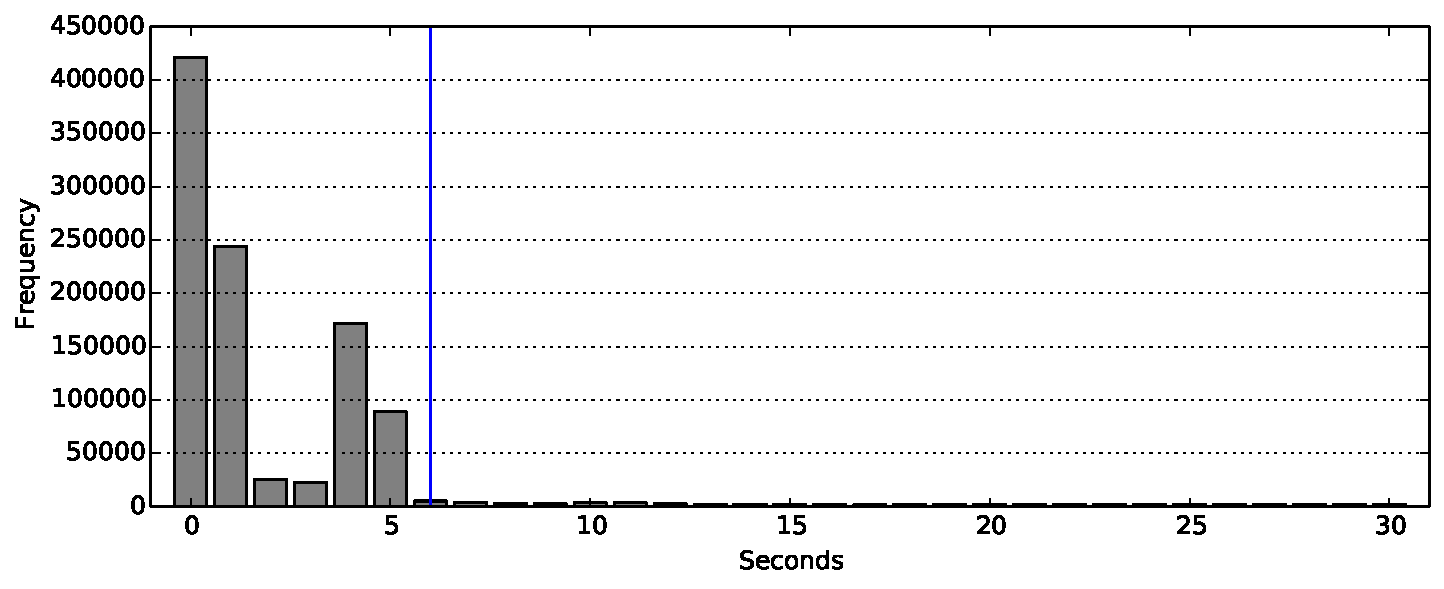
\includegraphics[width=\textwidth]{graphics/2015-08-14_17-46-44_faui1-246_timeout}
\caption{Duration of receiving one peer message}
\label{timeout-calibration}
\end{figure}

To assess a minimum timeout, an analysis with special configuration parameters was performed\footnote{Files: \texttt{2015-08-14\_17-46-44\_faui1-246.sqlite}, \texttt{2015-08-14\_17-46-44\_faui1-246\_timeout.txt}}. Here the maximum time used for receiving one message was recorded for every peer contact. These durations were rounded and the number of occurrences plotted in figure \ref{timeout-calibration}. For this task \config{network\_timeout} was set to 30 seconds to achieve most unbiased results. During this test at \numprint{977301} out of \numprint{1040817} peer contacts the maximum duration for receiving one message was below six seconds, which equals \numprint[\%]{93.9}.

\paragraph{\config{torrent\_complete\_threshold}}
\dots

\paragraph{\config{peer\_evaluation\_threads}}
\dots

TODO: Number of threads: workload plot

\section{Restrictions}

Restrictions and why this does not invalidate the results (hopefully, TBD):

\begin{itemize}
  \item No support for IPv6 on HTTP, UDP or DHT requests
  \item No support for the Micro Transport Protocol ($\mu$TP)
  \item No support for Peer exchange (PeX)
  \item No support for the Tracker exchange extension (BEP 28)
  \item No support for the BitTorrent Local Tracker Discovery Protocol (BEP 22)
  \item No BitTrorrent Protocol support for getting download progress info
  \item Drawback: One can only derive lower bounds from observing peers using the standard BitTorrent protocol
\end{itemize}


\section{Usage}
pymdht: It must me started seperately and is controlled automatically using a localhost Telnet connection. It could not be integrated directly, since it is written in Python version 2. The desired UDP node port and the Telnet control port must be given as arguments and should reflect the values written in the \emph{BitTorrent Download Analyzer's} configuration file. The typical command used here is \texttt{run\_pymdht\_node.py -{}-port=17000 -{}-telnet-port=17001}. It is sensible to check whether \emph{pymdht} has crashed before and after each analysis run to ensure complete results.

The main script, named \texttt{btda.py} can be controlled by using the following command line options.

\begin{description}
  \item[\texttt{-{}-active <threads>}] Actively contact and evaluate peers using the specified number of threads.
  \item[\texttt{-{}-passive}] Listen on the port specified in the configuration file for incoming connections and evaluate these peers.
  \item[\texttt{-{}-dht}] Integrate and control an already running \emph{pymdht} \cite{pymdht} DHT node using Telnet. The UDP port on which the node is running and the localhost Telnet port where \emph{pymdht} can be controlled are given via \config{dht\_node\_port} and \config{dht\_control\_port} respectively.
  \item[\texttt{-{}-debug}] Write log messages to the console instead of a file and include debug messages.
  \item[\texttt{-{}-help}] Show a help message and exit.
\end{description}
%%%%%%%%%%%%%%%%%%%%%%%%%%%%%%%%%%%%%%%%%%%%%%%%%%%%%%%%%%%%%%%%%%%%%%%%%%%%%%%%%%

\chapter{Evaluation}
Data collection with the BitTorrent Download Analyzer tool was performed on a virtual machine running Ubuntu 14.04 LTS with 1.0\,GB of RAM, a 3.4\,GHz processor and an own IPv4 address without NAT. The 15 chosen torrents were analyzed at once concurrently using \textbf{512 threads}. The analysis was performed from 11:11 am, August 15* to 11:11 am, August 17*, 2015. A time period of \textbf{48 hours} was chosen in order to detect patters during the day-night cycle. Necessary measures to ensure valid results were taken: The DHT node provided by \emph{pymdht} did not crash before or during the analysis. The BitTorrent Download Analyzer or any of its threads did not crash during the analysis and gave no relevant error message in the logfile.

\section{Choosing Torrents}
\begin{table}
\centering
\begin{tabular}{rllr}
\toprule
Rank & Site name & Domain name & Alexa Rank \\
\midrule
1 & Kickass Torrents & \texttt{kat.cr} & 116 \\
2 & ExtraTorrent.cc & \texttt{extratorrent.cc} & 335 \\
3 & Nyaa Torrents & \texttt{www.nyaa.se} & 399 \\
4 & Torrentz Search Engine & \texttt{torrentz.eu} & 464 \\
5 & The Pirate Bay & \texttt{thepiratebay.se} & 507 \\
6 & YTS & \texttt{yts.to} & 669 \\
7 & Rarbg & \texttt{rarbg.to} & 1,150 \\
8 & 1337x & \texttt{1337x.to} & 1,661 \\
9 & EZTV & \texttt{eztv.ch} & 1,831 \\
10 & torrentHound.com & \texttt{www.torrenthound.com} & 2,188 \\
11 & IPTorrents & \texttt{iptorrents.com} & 3,256 \\
12 & isoHunt & \texttt{isohunt.to} & 3,816 \\
13 & Bitsnoop P2P Search & \texttt{bitsnoop.com} & 4,293 \\
14 & Torrent Downloads & \texttt{www.torrentdownloads.me} & 4,315 \\
15 & LimeTorrents.cc & \texttt{www.limetorrents.cc} & 4,552 \\
16 & TamilRockers.net & \texttt{tamilrockers.com} & 4,586 \\
17 & Monova Torrent Search & \texttt{www.monova.org} & 4,843 \\
\bottomrule
\end{tabular}
\caption[Popular torrent directory sites according to \textsc{Alexa}]{Popularity of torrent directory sites according to \textsc{Alexa}'s \cite{alexa} global traffic ranking. Only sites with a rank below \numprint{5000} are listed. Data is accurate as of July 16, 2015.}
\label{torrentsites}
\end{table}

Due to the distributed nature of BitTorrent, there unfortunately is no complete list or for all torrents currently active. Thus external data about popularity of torrents is needed, even if there is no guarantee of correctness. So to determine most popular torrent directory sites the global traffic rankings by \textsc{Alexa Internet, Inc.} \cite{alexa} were consulted. The websites where \textsc{Alexa}'s ranking was looked up were collected through manual investigation using web search engines, relevant news sites and cross references between torrent sites. Table~\ref{torrentsites} shows the \numprint{17} sites found having an rank below \numprint{5000}.

\begin{table}
\centering
\begin{tabular}{rllrrr}
\toprule
ID & Site name & Torrent name & Size & Leechers & Seeders \\
\midrule
1 & Kickass Torrents & torrent\_name & 3.0\,GB & 42 & 23 \\
1 & Kickass Torrents & torrent\_name & 3.0\,GB & 42 & 23 \\
1 & Kickass Torrents & torrent\_name & 3.0\,GB & 42 & 23 \\
1 & Kickass Torrents & torrent\_name & 3.0\,GB & 42 & 23 \\
1 & Kickass Torrents & torrent\_name & 3.0\,GB & 42 & 23 \\
1 & Kickass Torrents & torrent\_name & 3.0\,GB & 42 & 23 \\
1 & Kickass Torrents & torrent\_name & 3.0\,GB & 42 & 23 \\
1 & Kickass Torrents & torrent\_name & 3.0\,GB & 42 & 23 \\
1 & Kickass Torrents & torrent\_name & 3.0\,GB & 42 & 23 \\
1 & Kickass Torrents & torrent\_name & 3.0\,GB & 42 & 23 \\
1 & Kickass Torrents & torrent\_name & 3.0\,GB & 42 & 23 \\
1 & Kickass Torrents & torrent\_name & 3.0\,GB & 42 & 23 \\
1 & Kickass Torrents & torrent\_name & 3.0\,GB & 42 & 23 \\
1 & Kickass Torrents & torrent\_name & 3.0\,GB & 42 & 23 \\
15 & Kickass Torrents & torrent\_name & 3.0\,GB & 42 & 23 \\
1 & Kickass Torrents & torrent\_name & 3.0\,GB & 42 & 23 \\
1 & Kickass Torrents & torrent\_name & 3.0\,GB & 42 & 23 \\
1 & Kickass Torrents & torrent\_name & 3.0\,GB & 42 & 23 \\
1 & Kickass Torrents & torrent\_name & 3.0\,GB & 42 & 23 \\
1 & Kickass Torrents & torrent\_name & 3.0\,GB & 42 & 23 \\
1 & Kickass Torrents & torrent\_name & 3.0\,GB & 42 & 23 \\
1 & Kickass Torrents & torrent\_name & 3.0\,GB & 42 & 23 \\
1 & Kickass Torrents & torrent\_name & 3.0\,GB & 42 & 23 \\
1 & Kickass Torrents & torrent\_name & 3.0\,GB & 42 & 23 \\
1 & Kickass Torrents & torrent\_name & 3.0\,GB & 42 & 23 \\
1 & Kickass Torrents & torrent\_name & 3.0\,GB & 42 & 23 \\
1 & Kickass Torrents & torrent\_name & 3.0\,GB & 42 & 23 \\
\bottomrule
\end{tabular}
\caption[List of torrent chosen for evaluation]{* List of the 20 most popular torrents according to meta-search engine \textsc{Torrentz} \cite{torrentz}. At the end are five torrents above \numprint[GB]{5} and five recently published torrents . Selection was made on August 42, 2015, 11:00. The \emph{ID} was chosen by the SQLite database used for storage during the analysis.}
\label{torrents}
\end{table}

Popular torrents were often found to be registered on multiple tracker sites, which leads to mostly identical top torrents across various torrent sites. For the definite selection of torrents, the meta-search engine \textsc{Torrentz} \cite{torrentz} was used: It monitors torrents from all other major torrent sites and provides sort and filter options by peer count, torrent age and size. Torrents in three size groups were chosen: The nine most popular torrents below \numprint[GB]{1}, the nine most popular torrents above \numprint[GB]{1} and the nine most popular torrents above \numprint[GB]{10}. These \textbf{27 torrents} are listed in table \ref{torrents}.

\section{Getting Addresses of Peers}
\begin{table}
\centering
\begin{tabular}{lrrrr}
\toprule
Source & Total & Unique & New & Unique per Hour \\
\midrule
Tracker server & 5 & 2 & 3\,\% \\
DHT network & 10 & 2 & 3\,\% \\
Incoming peers & 1 & 2 & 3\,\% \\
\bottomrule
\end{tabular}
\caption[Received peer addresses per source]{Total and unique received peer addresses per source. \emph{Tracker server} and the \emph{DHT network} are actively contacted for new peers. Values of \emph{incoming peers} only include peers whose download progress was evaluated successfully. The duration to calculate the \emph{unique per hour} value is \numprint[h]{48}*, as mentioned earlier.}
\label{unique-peers}
\end{table}

Peers from all sources were considered, namely from the tracker server, the DHT network and incoming connections. The number collected peer addresses in regards to their source is shown in table \ref{unique-peers}. Since the \emph{incoming peers} data point only includes peers when their download progress was successfully evaluated, the ratio of \numprint[\%]{95}* new incoming peers implies that $1-\numprint[\%]{95}=\numprint[\%]{5}$* of unique incoming peers contacted us a second time, despite not receiving any torrent data.

Summary plot

The progression during the analysis period of all peer requests is shown in appendix \ref{request-history}. The ratio between new and duplicate received peer address information settles fairly quickly*. \emph{incoming-duplicate} is actually good.

\section{Evaluating Peer's Download Progress}
\begin{table}
\centering
\begin{tabular}{llrr}
\toprule
Event & Reason & Quantity & Share per Event \\
\midrule
First contact & timed out & 1653 \\
& [Errno 111] Connection refused & 420 \\
& Socket connection broken & 317 \\
& [Errno 104] Connection reset by peer & 47 \\
& [Errno 113] No route to host & 26 \\
& \emph{Total} & 4321 \\
\midrule
Later contact & Socket connection broken & 265 \\
& timed out & 27 \\
& [Errno 111] Connection refused & 6 \\
& [Errno 104] Connection reset by peer & 2 \\
& \emph{Total} & 4321 \\
\midrule
Incoming peer & Peer speaks unknown protocol & 891 \\
& timed out & 353 \\
& [Errno 104] Connection reset by peer & 9 \\
& Socket connection broken & 7 \\
& \emph{Total} & 4321 \\
\bottomrule
\end{tabular}
\caption[Reasons for failed peer evaluation]{Reasons for failed peer valuations during the analysis process. \emph{Event} describes the point in the evaluation process, when the problem occurred. \emph{First} and \emph{later contact} are performed when actively contacting collected peer addresses, while a peer must be contacted once successfully to be contacted another time. An \emph{incoming peer} represents an incoming connection on the BitTorrent listening port.}
\label{connection-failure}
\end{table}

Define failure

Failure reasons: Unsuppored client (mTP), probably not, see Client Analysis, probably bad/out of date peer address data

Failure rate per source out of scope

Total unique active success from peer database

Peer addresses received via DHT and tracker requests were contacted continuously. \numprint[\%]{0} of contacted peers failed when contacted for the first time. Of the peers contacted successfully once, \numprint[\%]{0} failed later.

\section{Counting Confirmed Downloads}
The timeline of confirmed downloads and downloads reported by the tracker server in scrape requests is shown in one hour steps in figure \ref{downloads}.

Map: Distribution of downloads (TODO)

\section{Peer's Analysis}
\subsection{Download Speed}
TODO: Graph of speed per country with standard derivation indicators, n>=10 per country

todo: Map of Distribution of download speeds

\subsection{BitTorrent Clients}
TODO: Table of frequency of BT clients

\subsection{Peer's Host Names}
TODO: Table: Examine hostnames by ISP or seedbox provicers
%%%%%%%%%%%%%%%%%%%%%%%%%%%%%%%%%%%%%%%%%%%%%%%%%%%%%%%%%%%%%%%%%%%%%%%%%%%%%%%%%%

\chapter{Conclusion and Future Work}
\dots
%%%%%%%%%%%%%%%%%%%%%%%%%%%%%%%%%%%%%%%%%%%%%%%%%%%%%%%%%%%%%%%%%%%%%%%%%%%%%%%%%%

\appendix
\chapter{Collected Data}
\section{Development of received peer addresses per source}
\label{request-history}
\includegraphics[width=\textwidth, page=1]{graphics/2015-07-18_21-57-15_faui1-246_source}\\
\includegraphics[width=\textwidth, page=2]{graphics/2015-07-18_21-57-15_faui1-246_source}\\
\includegraphics[width=\textwidth, page=3]{graphics/2015-07-18_21-57-15_faui1-246_source}\\
\includegraphics[width=\textwidth, page=4]{graphics/2015-07-18_21-57-15_faui1-246_source}\\
\includegraphics[width=\textwidth, page=5]{graphics/2015-07-18_21-57-15_faui1-246_source}\\
\includegraphics[width=\textwidth, page=6]{graphics/2015-07-18_21-57-15_faui1-246_source}\\
\includegraphics[width=\textwidth, page=7]{graphics/2015-07-18_21-57-15_faui1-246_source}\\
\includegraphics[width=\textwidth, page=8]{graphics/2015-07-18_21-57-15_faui1-246_source}

\section{Confirmed and server reported download numbers}
\label{downloads}
\includegraphics[width=\textwidth, page=1]{graphics/2015-07-18_21-57-15_faui1-246_download}\\
\includegraphics[width=\textwidth, page=2]{graphics/2015-07-18_21-57-15_faui1-246_download}\\
\includegraphics[width=\textwidth, page=3]{graphics/2015-07-18_21-57-15_faui1-246_download}\\
\includegraphics[width=\textwidth, page=4]{graphics/2015-07-18_21-57-15_faui1-246_download}\\
\includegraphics[width=\textwidth, page=5]{graphics/2015-07-18_21-57-15_faui1-246_download}\\
\includegraphics[width=\textwidth, page=6]{graphics/2015-07-18_21-57-15_faui1-246_download}\\
\includegraphics[width=\textwidth, page=7]{graphics/2015-07-18_21-57-15_faui1-246_download}\\
\includegraphics[width=\textwidth, page=8]{graphics/2015-07-18_21-57-15_faui1-246_download}
%%%%%%%%%%%%%%%%%%%%%%%%%%%%%%%%%%%%%%%%%%%%%%%%%%%%%%%%%%%%%%%%%%%%%%%%%%%%%%%%%%

\printbibliography[heading=bibintoc]
\end{document}
